\documentclass[a4paper]{scrartcl}
\usepackage[english]{babel}
\usepackage[utf8]{inputenc}
\usepackage{hyperref}
\usepackage{tikz}


\begin{document}

\title{Lbx File Format}
\author{Marco Kull - \href{mailto:marco_kull@web.de}{marco\_kull@web.de}}\date{}
\maketitle
\thispagestyle{empty}

The lbx file format is a simple container that consist of a header followed by multiple concatenated files. It is used in some old DOS games developed by SimTex:
\begin{itemize}
\item[-] Master of Magic
\item[-] Master of Orion 1
\item[-] Master of Orion 2
\item[-] 1830: Railroads \& Robber Barons
\end{itemize}

Some files in these games have a .LBX suffix but aren't real lbx file containers. This also seems to be true for all lbx files contained in StarLords - a precessor of Master of Orion 1.\\\\
A lbx file can be read like this:
\begin{flushleft}
\begin{tabular}{|l|l|l|l|}
\hline
\textbf{Field} & \textbf{Size} & \textbf{Description}\\ 
\hline \hline
n & 2 bytes & Number of files contained in lbx archive.\\\hline
offset & 4 bytes & n +1 offsets.\\\hline
data & (offset[i+1]-offset[i]) bytes & Raw file data.\\\hline
\end{tabular}
\end{flushleft}

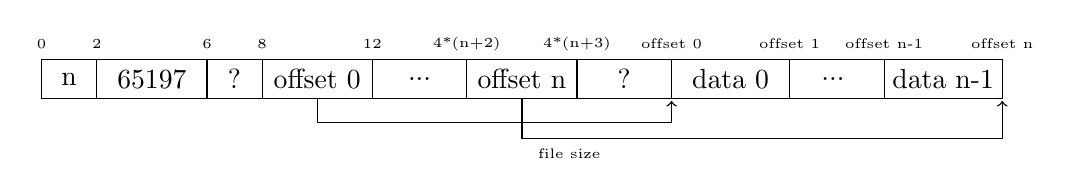
\begin{tikzpicture}
\draw (0,2) -- (12.2,2) -- (12.2, 2.5)  -- (0, 2.5) -- (0,2);
	
\node[font=\tiny] at (0,2.7) {0};
	 
\node at (0.35,2.25) {n};
\node[font=\tiny] at (0.7,2.7) {2};
\draw (0.7, 2.5) -- (0.7, 2);
		
\node at (1.4,2.25) {65197};
\node[font=\tiny] at (2.1,2.7) {6};
\draw (2.1, 2.5) -- (2.1, 2);
	
\node at (2.45,2.25) {?};
\node[font=\tiny] at (2.8,2.7) {8};
\draw (2.8, 2.5) -- (2.8, 2);
	
\node at (3.5,2.25) {offset 0};
\node[font=\tiny] at (4.2,2.7) {12};
\draw (4.2, 2.5) -- (4.2, 2);
	
\node at (4.8,2.25) {...};
\node[font=\tiny] at (5.4,2.7) {4*(n+2)};
\draw (5.4, 2.5) -- (5.4, 2);
	
\draw (6.8, 2.5) -- (6.8, 2);
\node at (6.1,2.25) {offset n};
\node[font=\tiny] at (6.8,2.7) {4*(n+3)};
\draw (6.8, 2.5) -- (6.8, 2);
	
\node at (7.4,2.25) {?};
\node[font=\tiny] at (8,2.7) {offset 0};
\draw (8, 2.5) -- (8, 2);
	
\node at (8.75,2.25) {data 0};
\node[font=\tiny] at (9.5,2.7) {offset 1};
\draw (9.5, 2.5) -- (9.5, 2);
	
\draw (10.7, 2.5) -- (10.7, 2);
\node at (10.05,2.25) {...};
\node[font=\tiny] at (10.7,2.7) {offset n-1};

\node at (11.45,2.25) {data n-1};
\node[font=\tiny] at (12.2,2.7) {offset n};

\draw[arrows=->,line width=.5pt](3.5, 2)--(3.5,1.7)--(8,1.7)--(8,1.975);
%\node[font=\tiny] at (3.9,1.5) {2048};
\draw[arrows=->,line width=.5pt](6.1, 2)--(6.1,1.5)--(12.2,1.5)--(12.2,1.975);
\node[font=\tiny] at (6.7,1.3) {file size};
\end{tikzpicture}
\\\\
The meaning two bytes between the signature (65197) and the first offset are unknown. Also sometimes there's a space between the last offset and the beginning of the file data containing data that doesn't seem to make any sense. In Master of Orion 2 the first offset is always 2048.
\end{document}

